% !TeX encoding = utf8
% !TeX spellcheck = en_US

\section{Results}
As can be seen in Figure \ref{fig:filtvsunfilt}, after applying the evaluated Chebyshev Type II IIR filter, the unwanted noise has essentially been fully removed from the signal and a clean PPG signal is obtained. The Chebyshev Type II IIR filter was chosen because of the monotonic pass-band and due to the attenuation in the band-stop region being higher compared to the equiripple FIR filter.

\begin{figure}[H]
	\centering
	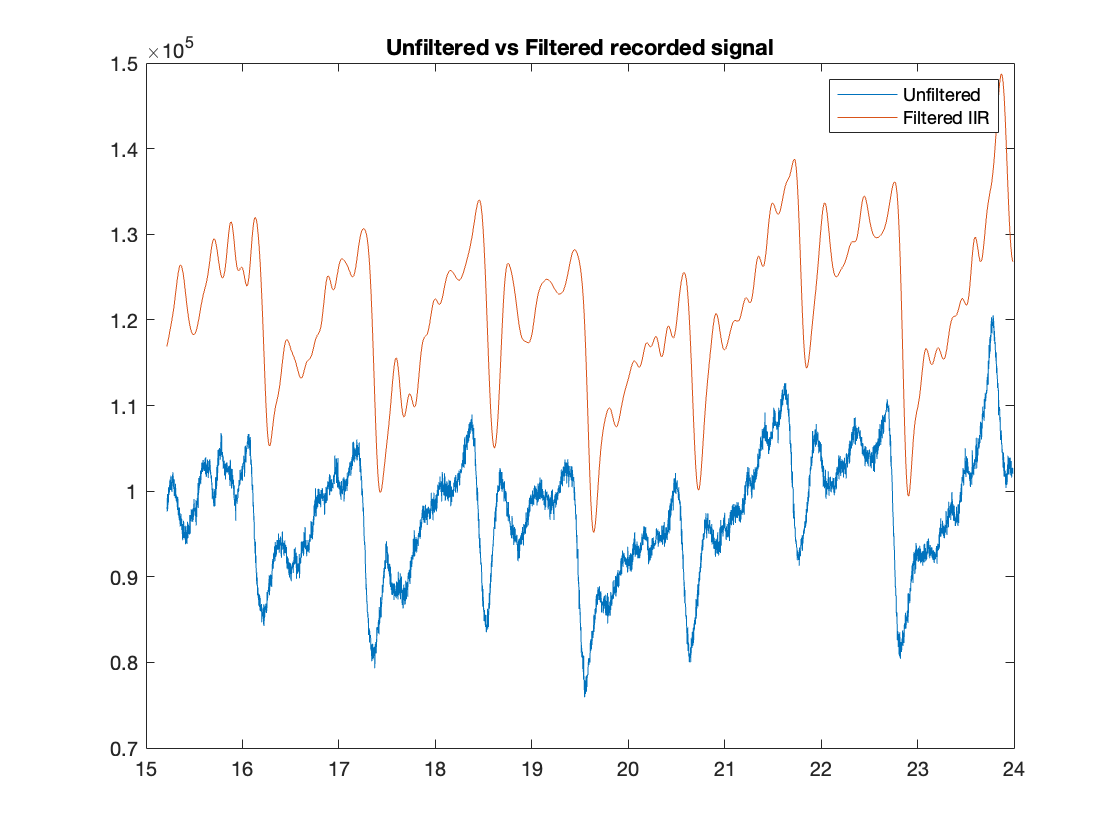
\includegraphics[width=\linewidth, trim={2.5cm, 1cm, 2cm, 1cm}, clip]{Figures/filteredvsunfiltered.png}
	\caption{The unfiltered recorded signal compared to the filtered recorded signal.}
	\label{fig:filtvsunfilt}
\end{figure}

Once the filtered PPG signal was obtained, the heartbeat peak detection algorithm was applied. In a range of 90\,seconds, the algorithm was successfully able to detect 82 true peaks (i.e. 82 true positives) but failed to detect 2 true peaks (i.e. 2 false negatives). This results in an overall sensitivity of 97.6\% for the peak detection algorithm, as calculated by Equation \eqref{eqn:accuracyEquation}. Additionally, this results in a heartbeat of roughly 55\,bpm, which corresponds to an expected resting heartbeat.


%The results of the evaluation can be found in Table \ref{tab:peacks_detected}.
%\begin{table} [h]
%	\caption{Algorithm evaluation in MATLAB.}
%	\centering % Horizontally center the table
%	\begin{tabularx}{\linewidth}{X|X|} % Manually specify column alignments with L{}, R{} or C{} and widths as a fixed amount, usually as a proportion of \linewidth
%		\toprule
%		Evaluation & \# of peaks \\
%		\midrule
%		Manually & 84 \\
%		Algorithm  & 82 \\
%		\bottomrule
%	\end{tabularx}
%	\label{tab:peacks_detected}
%\end{table} 

When the algorithm was subsequently implemented on the microcontroller, it failed to detect any peaks. Despite extensive efforts, a bug in the microcontroller implementation hindered the evaluation process. Due to time constraints, this bug could not be identified and resolved within the given project timeline. Consequently, while the algorithm shows promise based on initial evaluations, further debugging and refinement are necessary to ensure its functionality on the microcontroller platform.
